%!TEX root = problems.tex

\printanswers

\noindent
This is the introduction~\cite{knuthwebsite}.

\begin{questions}

\question
Is this a question?
\begin{solution}
\begin{minted}{python}
if it is:
  print answer
\end{minted}
\end{solution}


\question
Is this another question?
\begin{solution}
Another solution.
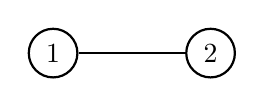
\begin{tikzpicture}
\begin{scope}[every node/.style={circle,thick,draw}]
\node (1) at (0,0) {1};
\node (2) at (2,0) {2};
\end{scope}
\begin{scope}[every edge/.style={draw=black,thick}]
\path (1) edge (2);
\end{scope}
\end{tikzpicture}
\end{solution}


\question
Here's a table:
\begin{table}[H]
  \centering
  \begin{tabular}{x{1.5cm}x{1.5cm}x{1.5cm}x{1.5cm}x{1.5cm}}
    \toprule
    State	& Input	& Write & Move & Next \\
    \midrule
    \multirow{3}{*}{1}
      & B &	0 &	R & 2 \\
      & 0	& 0 & R &	2 \\
      & 1	& 0 &	R &	2 \\
    \midrule
    \multirow{3}{*}{2}
      & B & 1 & R & 1 \\
      & 0	& 1 &	R &	1 \\
      & 1 & 1 &	R &	1 \\
    \bottomrule
    \hline
  \end{tabular}
\end{table}


\end{questions}
